\autsection{Technical Plan}{Nelián Colón, Samuel Rodríguez and Daniel Santiago}

\subsection{Web Application}

Panda Code Reviews is a fully hosted web application. The web application
includes many parts, the main of these are the front end and the back end. The
front end is what the user sees and interacts with directly. It is very
important to design the front end with ease of use in mind, and almost equally
important is designing the interface with a clean and modern look. The back end
is the underlying software that manages the communication between the front end
interface and the database, repository manager and testing framework. The front
end and the back end are connected in various parts, so this must be properly
designed for ensuring compatibility and hassle-free communication. For example,
data passing between the database and the front end through the back end must
be concise, so a standard object model should be used. It is discussed in the
following sections the usage of JSON objects for this purporse. Additionally,
the URL Endpoints of the application must be specified for compatibility
between the front end and the back end.

\subsection{Front end}

As mentioned earlier, it is very important to design the front end interface
with ease of use in mind, and it is also very important to design the interface
with a clean and modern look. The Model-View-Controller (MVC) pattern is being
followed for developing the front end. The idea of the MVC pattern is to have an
good organization in the code between managing the application's data (model),
the application's logic (controller), and the application's presentation (view).
The view gets data from the model to display to the user. When a user interacts
with the application, the controller changes data in the model, and the data
gets passed from the model to the view so that it is displayed to the user. In
the case of Panda Code Reviews, the view of the application is the Document
Object Model (DOM) of the web pages. The controller of the application is
JavaScript code that uses AngularJS, and the model data is all stored in JSON
objects.

One of the most difficult tasks in developing the front end of the application
is ensuring good compatibility between the model, the view and the controller.
AngularJS makes this compatibility easier by providing a type of templating
engine in the client side. It allows for automatic refreshing of data. For
example, if the controller of the application changes the model data, AngularJS
automatically refreshes the view so that it gets displayed to the user. And if
the view is changed by the user, AngularJS can automatically update the model.

\subsubsection{View}

The view is being handled by HTML and CSS. Panda Code Reviews uses Bootstrap, an
open source front end framework for faster and easier development of the front
end's view. It provides many CSS classes for easily templating the web pages. It
is also highly customizable, and provides a JavaScript plugin interface for
enabling animations and other features like component pinning. These plugins
might be activated by the controller or by other means such as after a page
loads.

\subsubsection{Controller}

The controller of the front end is being developed in JavaScript. JavaScript is
implemented by all major browsers and provides a very comprehensive standard
library for manipulating elements of the DOM and registering event listeners.
JQuery, a comprehensive JavaScript library, is being used for simplifying and
reusing many routines. Also, AngularJS is being used for simplifying
communication between the model, the view and the controller. More will be
discussed about AngularJS in the next section.

\subsubsection{Model and Communication}

The model of the application is embedded in the controller and specified in the
database, which the front end has no direct access to. Instead, the front end
will communicate with the back end through a REST API, and the back end will
answer the front end's query with JSON objects. AngularJS, an open source
templating framework, will be used for simplifying the communications between
the front end's controller and model. AngularJS will also be used for
communicating with the back end through its REST API. When the user interacts
with the front end's view, AngularJS responds by changing the model in the front
end, which will then call the necessary controller functions that will
communicate with the back end through its REST API. The back end will respond to
the controller's query with JSON objects, and AngularJS will manage the change
of data between the controller, the model and the view. AngularJS is also highly
modifiable, so some functionality is overriden so that it better suits Panda
Code Review's functionalities.

\subsubsection{Views}
As the time of this writing, the team has developed some static web pages with
HTML4/5 and Bootstrap CSS. This doubles as part of the implementation of the
front end and as Mockups creation for the design phase. The application views
that have been planned by the team follows. Use case diagrams can be found in 
Appendix~\ref{sec:useCase} and descriptions can be found in 
Appendix~\ref{sec:useCases}. Screenshots of what the users is
expected to see are found in Appendix~\ref{sec:mockups}.

\begin{enumerate}

\item \textbf{Site Home Page:} The site homepage will include information and
marketing information about Panda Code Reviews and the services that it offers.
It will also include links for logging in and signing up. If the user is
already logged in, it will also include links for accessing his account
home page and general account settings.

\item \textbf{Login and Sign Up:} The login screen and sign up screen asks for
the users e-mail and password. If the user clicks the sign up button, it will
also ask for the user's name and for a password retype.

\item \textbf{Account Home:} The account home will show different things
depending on the user. If the user is a student, the account home will show the
enrolled courses and will also contain a button for enrolling new courses. Each
course will also contain a snippet of the assignments that are due and the
dates at which they are due. The student could click on the course name to see
more information about the course, and he could also click on the due
assignment names to see more information about the assignments. In the case of
a professor, he would be able to see the list of courses, and could also create
a new course. The professor would also be able to see the amount of students
enrolled in the course and the names, contact emails, and summary of grades of
each student.

\item \textbf{Create Course:} The professor is the only one that can see the
create course view. This view is included as part of the account home of the
professor, it is a drop down that asks for the new course's name. After
creating the course, the professor can edit it and add students.
% todo, there is something missing here.

\item \textbf{View Course:} Students and professors can view the courses. in
case of the student, he will be able to see basic information about the course,
like course title, number, semester, and year. He can also see a summary of his
grade, his assignments, and his submissions. He can also see contact
information of his professor in a glance. A professor can see with great detail
the amount of students in the course, and the assignments that he currently has
in the course. He can also edit and delete the course from this veiw, and can
create new assignments to add to the course.

\item \textbf{Enroll Course:} The student can easily enroll in a course in the
enroll course view which is part of the student's account home view. This view
is a drop down that only asks for the courses name. This is a searching
feature. As the student types up the name, it will instantly provide results.
The student can then select a course and enroll in it.

\item \textbf{Create Assignment:} The professor can create an assignment in his
course view. This view is a drop down, where the professor can add the
name and the due date of the assignment.

\item \textbf{Assignment Information:} Professors and students can see this
view. For the students, the information view will contain the description, the
instructions for completing the assignment, the due date, the student's score,
and the last submission date. The professor also has the ability to view the
scores of every student, and can also edit and delete information from the
assignment. A student can only view the information of the assignment and can
only view his own grade.

\item \textbf{Assignment Submissions:} Both students and professors can see the
assignment submissions. The difference is that the students can only see their
own submissions, whereas the professor can see the submissions of every single
student. the submission information will include the hash id, the student's
name, the submit date, the result of the suybmission, the score, the compile
time of the submission, and the run time of the submission. The professor will
also have an additional button that allows him to override the grade of a
student.

\item \textbf{Assignment Test Cases:} Both students and professors can see the
assignment test cases, the difference is that the professor can add, edit and
delete test cases, whereas the student can only view them and develop his
assignment accordingly.

\item \textbf{Assignment Repositories:} Both the students and the professors
can see the repositories, but the student can only see his own repositories
whereas the professors can see the repositories of every student.

\item \textbf{Add test cases:} The professor can add test cases in the
assignment test cases view. This will ask for the input of the test case and
the expected output.

\item \textbf{Grade:} Both students and professor can see grades. The students
can see their own grade from the assignment view and from the course view. The
student will be able to view grade from specific assignments or total grades
for specific courses. The professors can see the grades of every student for
his courses and assignments. He can also modify their grades.

\item \textbf{Account Profile:} Both students and professors will be able to
see the account profiles.

\item \textbf{Account Security:} Both students and professors will be able to
see their account securities information. This will include the ability to
change their passwords and view and add ssh keys.


\end{enumerate}

\subsection{Back end}

The back end is the underlying server side software that manages the
communication and flow between the front end and the database server, the
repository manager, and the testing framework. The front end sends requests for
data to the back end using its REST API. The back end then proceeds with
establishing a connection to the MongoDB database server and then passing the
query's result to the front end. The database server returns query results with
JSON objects, and the back end does not have to translate this information in
any way, since the front end also uses JSON objects as discussed in the earlier
sections. The back end is also responsible of instantiating the sand boxes where
the submitted code and test cases will run. This is also invoked by orders of
the users when they interact with the front end of Panda Code Reviews.

% usar palabra fancy: serialization and deseriaization. Si fuera SQL, habria
% que hacer todas esas cosas.

\subsubsection{Node.js}

% a~nadir  footnotes explicando.

The back end service is being built in JavaScript using Node.js. Node.js is a
platform built on Google Chrome's Open Source V8 JavaScript runtime engine for
easily building fast and scalable network and server-side applications. It uses
JavaScript as its scripting language and achieves high throughput via an event
driven, non-blocking I/O model on a single-threaded event loop. It also contains
a built-in HTTP server library, which allows for easy deployment of a web server
without the need of external HTTP servers like Apache, Lighttpd or Nginx.
Node.js poses additonal ease of use when it comes to interacting with MongoDB,
since it uses JSON-style documents as well. This means that no additional
library or wrapper is needed to communicate with the database.

\subsubsection{GitLab}

GitLab is open source software to help developers collaborate on code. It can be
used to create projects and repositories and manage access.

\subsubsection{Endpoints}

An endpoint of a software designed with the service-oriented architecture (SOA)
pattern is the entry point of a particular service that the software provides,
where a service stands for a single activity. In the case of Panda Code Reviews,
the Endpoints are specified by the URLs that the client's browser must access in
order to receive the individual services from the back end that make up the web
application. The user need not know or specify these Endpoints, since the web
application's front end will already provide them to the client's browser. These
Endpoints are designed using the RESTful (representational state transfer) web
design architecture. The Endpoint URLs will be prefixed by api/ in order to
clearly separate the URLs that are intended to be part of the RESTful API of the
backend and the URLs that are intended to be accessed as part of the front end
application. The following tables specify the endpoints' method, url and
description.

\setlength{\extrarowheight}{1.5pt}
    \begin{longtable}{|c|c|c|m{4cm}|}
 \caption{Users Endpoints\label{tab:addlabel}} \\
     \hline
    
    \centering  Method & Path & Query String & Description \\
    \hline \hline \endfirsthead
    
         \hline

  \centering  Method & Path & Query String & Description \\
    \hline \hline \endhead
    
    \endfoot  
    GET   & /users & ?course=\$cid & {Gets list of users} \\ \hline
    GET   & /users/\$uid &       & {Gets data from user \$uid} \\ \hline
    POST  & /users &       & {Creates users with JSON pyaload} \\ \hline
    PUT   & /users/\$uid &       & {Updates user \$uid data with JSON payload} \\ \hline
    DELETE & /users/\$uid &       & {Soft delete user \$uid} \\ \hline
    GET   & /users/\$uid/courses & ?year=\$y\&semester=\$s & {Gets courses of user \$uid} \\ \hline
    GET   & /users/\$id/assignments & ?course=\$cid & {Gets assigments of user \$uid} \\ \hline
    GET   & /users/\$id/submissions & ?assigment=\$aid\&course=\$cid & {Gets submissions of user \$uid} \\ \hline
\end{longtable}

\setlength{\extrarowheight}{1.5pt}
    \begin{longtable}{|c|c|c|m{4.5cm}|}
 \caption{Courses Endpoints\label{tab:addlabel}} \\
     \hline
    
    \centering  Method & Path & Query String & Description \\
    \hline \hline \endfirsthead
    
         \hline

    \centering  Method & Path & Query String & Description \\
    \hline \hline \endhead
    
    \endfoot 
    GET   & /courses & ?year=\$y\&semester=\$s & {Gets list of courses} \\ \hline
    GET   & /courses/\$cid &       & {Gets data from course \$cid} \\ \hline
    POST  & /courses &       & {Creates course with JSON payload} \\ \hline
    PUT   & /courses/\$cid &       & {Updates course \$cid data with JSON pyaload} \\ \hline
    DELETE & /courses/\$cid &       & {Soft delete course \$cid} \\ \hline
    GET   & /courses/\$cid/users & ?isGrade=\$bool & {Gets users of course \$cid} \\ \hline
    POST  & /courses/\$cid/users/\$uid &       & {Adds user \$uid to course \$cid} \\ \hline
    DELETE & /courses/\$cid/users/\$uid &       & {Removes user \$uid from course \$cid} \\ \hline
    GET   & /courses/\$cid/assignments &       & {Gets assigments of course \$cid} \\ \hline
    GET   & /courses/\$cid/submissions & ?assignment=\$aid & {Gets submissions of course \$cid} \\ \hline
\end{longtable}

\setlength{\extrarowheight}{1.5pt}
    \begin{longtable}{|c|c|c|c|}
 \caption{Assignments Endpoints\label{tab:addlabel}} \\
     \hline
    
    \centering  Method & Path & Description \\
    \hline \hline \endfirsthead
    
         \hline

    \centering  Method & Path & Description \\
    \hline \hline \endhead
    
    \endfoot 
    GET   & /assignments & {Gets a list of assignments} \\ \hline
    GET   & /assignments/\$aid & {Gets data from assignment \$aid} \\ \hline
    POST  & /assignments & {Creates assignment from JSON payload} \\ \hline
    PUT   & /assignments & {Updates assignment \$aid data with JSON payload} \\ \hline
    DELETE & /assignments/\$aid & {Soft delete assignment \$aid} \\ \hline
    POST  & /assignments/\$aid/test & {Creates a test case from assignment \$aid} \\ \hline
    DELETE & /assignments/\$aid/test/\$tid & {Deletes test case \$tid from assignment \$aid} \\ \hline
\end{longtable}

\setlength{\extrarowheight}{1.5pt}
    \begin{longtable}{|c|c|m{10cm}|}
 \caption{Submissions Endpoints\label{tab:addlabel}} \\
     \hline
    
    \centering  Method & Path & Description \\
    \hline \hline \endfirsthead
    
         \hline

    \centering  Method & Path & Description \\
    \hline \hline \endhead
    
    \endfoot 
    GET   & /submissions & {Gets a list of submissions} \\ \hline
    GET   & /submissions/\$sid & {Gets data from submissions \$sid} \\ \hline
    POST  & /submissions & {Creates submissions from JSON payload. Endpoint that queues code for evaluation} \\ \hline
\end{longtable}


\subsubsection{Codeworkers}

\subsection{Database}

The database is used for storing all required information about the system and
its users.

\subsubsection{MongoDB}

MongoDB is a cross-platform document-oriented database system. It is classified
as a NoSQL database which provides a mechanism for storage retrieval that is not
as constrained as relational databases like MySQL or PostgreSQL. MongoDB
features JSON-style (JavaScript Object Notation) documents with dynamic schemas,
which allows simpler and quicker development. A dynamic schema approach enables
flexibility for quickly changing applications, and the JSON style documents
provide a unified language for passing database objects between the Node.js
backend and the front end, both written entirely in Javascript. MongoDB is the
leading NoSQL DBMS, it is more stable than its closest competitor Redis.

\subsubsection{Entity-Relationship Diagram}

The collections have been defined following two different approaches: the
standard ER diagram that defines entities and the relationships with each other
and a JSON-like diagram that better models MongoDB's Documents and Collections.
Overall, we created structures for users (Administrators, Professors, Students
and TAs), courses, assignments and submissions.

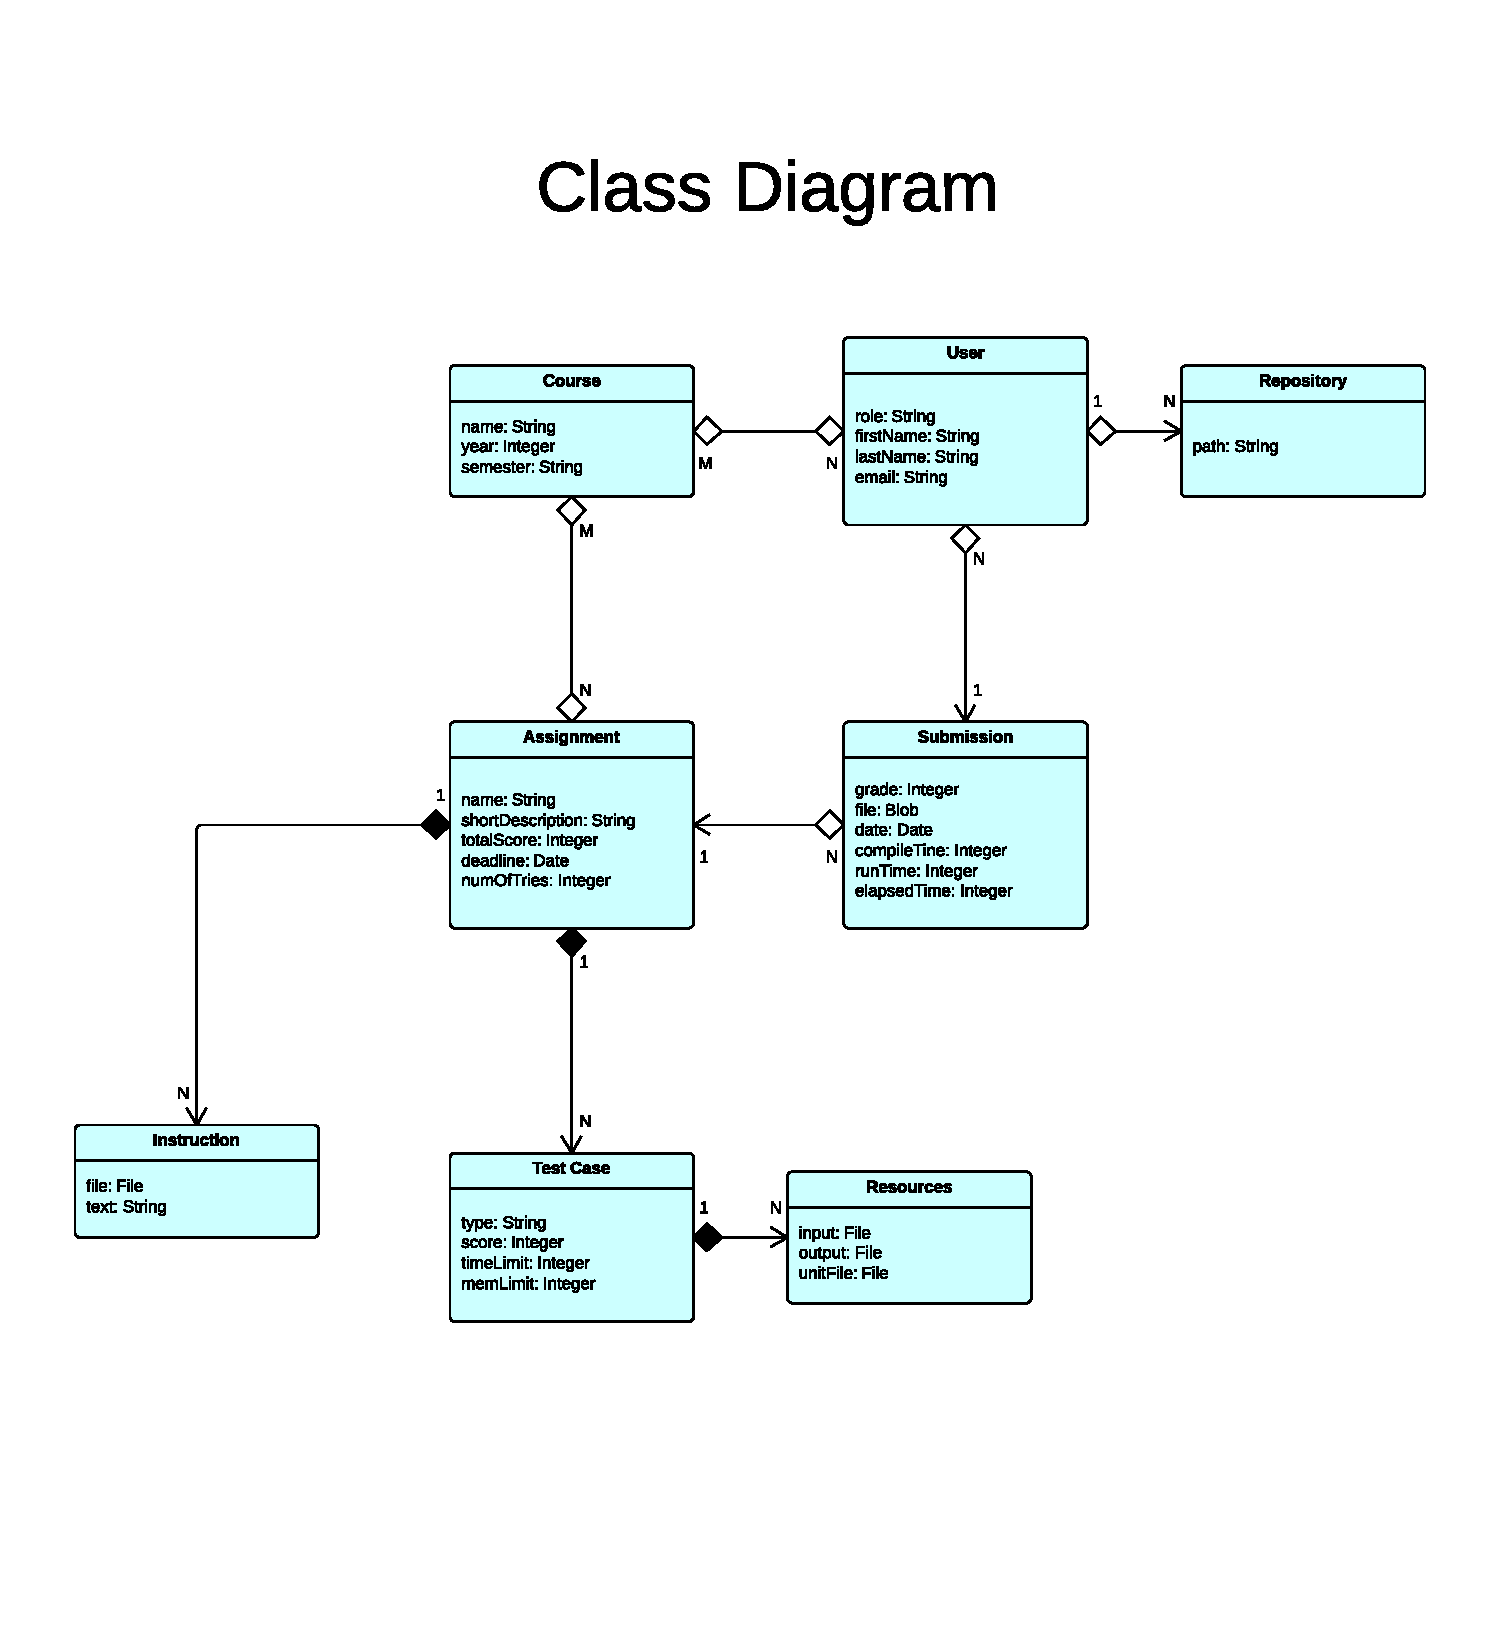
\includepdf[pages={-}]{img/class_diagram.pdf}


\subsection{Deployment}

Continuous development has been set up in the deployment server colocated at
Amazon's EC2 infrastructure. This enables an always working version hosted in
the cloud which gets automatically deployed whenever a developer pushes code to
the master branch in Git. When the latest version is pushed, the Node Package
Manager (NPM) runs code tests to make sure that the latest push is healthy. If
it passes the tests, the server is shut down, any new dependencies are installed
with NPM, and the server is restarted with the new changes in effect. This all
happens automatically.

% This is the overview of the front end and back end architecture.
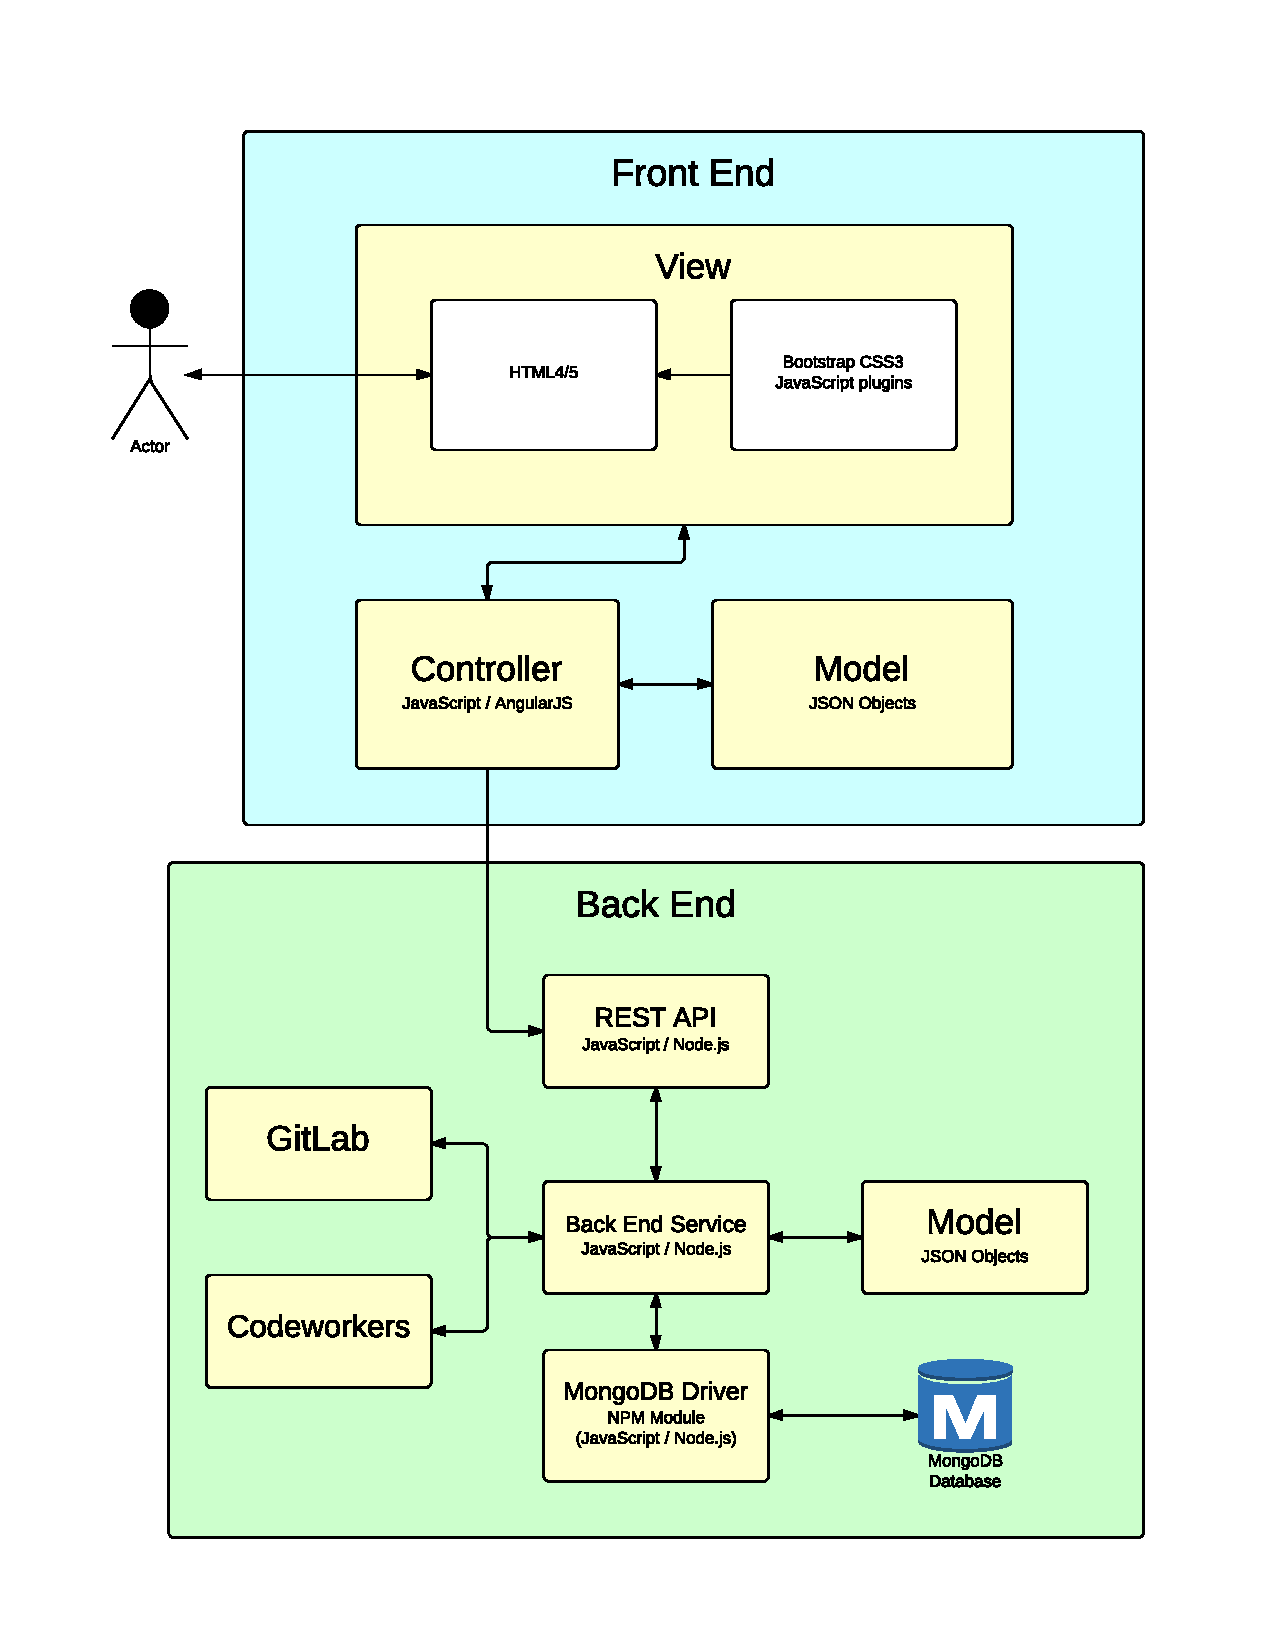
\includepdf[pages={-}]{img/tech_archi.pdf}

%presents and describes design alternatives, and justifies all the choices made

%presents and describes system architecture

%present progress in the design with technical diagrams and description of system components (appendices required for calculations, and detailed documentation diagrams and descriptions)

%analyzes and justifies any departures with respect to original plan

%presents snapshots or other evidences

%check list:

%present system design overview
%present sys conceptual design (how it will look like)
%present software architecture
%present component description
%present user interface
%presents software progress assessment
%presents class diagrams
%presents software design justications
%presents communication interfaces